\documentclass[a4paper]{article}

\usepackage[utf8]{inputenc}
\usepackage[T1]{fontenc}
\usepackage{lmodern}
\usepackage[brazil]{babel}
\usepackage[a4paper,margin=2.5cm]{geometry}
\usepackage{amsmath}
\usepackage{graphicx}
\usepackage{booktabs}
\usepackage[hidelinks]{hyperref}

\graphicspath{{figuras/}}

\begin{document}

\begin{titlepage}
\centering
\vspace*{3cm}
{\large Universidade Federal de Pernambuco\\Centro de Informática\\[4pt]CIN0020 Sinais e Sistemas, 2026.2\par}
\vspace{3cm}
{\LARGE\bfseries Análise de sinais de vibração de drones com hélices saudáveis e defeituosas\par}
\vspace{0.8cm}
{\large Relatório parcial\par}
\vspace{3cm}
{\large Carolina Santiago de Medeiros (csm6)\\Karolyne Bezerra Rocha (kbr)\\Milla Rwana de Araújo Silva (mras3)\par}
\vfill
{\large Recife, novembro de 2026\par}
\end{titlepage}

\begin{abstract}
Analisamos sinais reais de aceleração do conjunto DronePropB para comparar hélices saudáveis e defeituosas. Os registros de um acelerômetro piezoelétrico foram divididos em janelas de 1~s, das quais extraímos características no tempo e na frequência. As medidas de intensidade dependem sobretudo da velocidade e não indicam mais vibração no defeito de forma consistente, enquanto o espectro mostra que a vibração é formada pela rotação e seus harmônicos, que o defeito redistribui a potência entre eles e que a hélice danificada gira um pouco mais devagar.
\end{abstract}

\section{Introdução}

Danos nas hélices de um drone podem alterar a intensidade e o conteúdo em frequência das vibrações que ele produz. Neste relatório parcial de um projeto ainda em andamento, caracterizamos sinais de aceleração de hélices saudáveis e defeituosas nos domínios do tempo e da frequência, extraímos características por janela e discutimos quais delas distinguem as condições, como preparação para a etapa de classificação. Ao longo do texto indicamos qual resultado da disciplina justifica cada passo, citando as notas de aula pelo número da aula e do slide.

\section{Dados e preparação}

O DronePropB~\cite{dataset} reúne ensaios em solo de um drone comercial com hélice saudável (F0) ou com três tipos de defeito (F1, F2 e F3) em três severidades (SV1 a SV3), em três velocidades (SP1 a SP3) e organizados em configurações (C1 a C4), provavelmente experimentos diferentes. Cada arquivo traz o sinal de um acelerômetro piezoelétrico de um eixo, amostrado a $f_s = 10$~kHz e sem unidade registrada (usamos unidades arbitrárias, u.a.), e o de uma IMU de três eixos a 1~kHz. Escolhemos o piezo porque sua frequência de Nyquist, 5~kHz, cobre com folga a rotação e seus harmônicos e ainda permite demonstrar o aliasing.

Selecionamos a configuração C1 completa (Tabela~\ref{tab:registros}). Os saudáveis de C2 são cópias idênticas dos de C1, mas os defeituosos não; como não se sabe a qual experimento esses saudáveis pertencem, usamos C2 só como checagem (Seção~6). C3 e C4 têm registros curtos ou só saudáveis. As comparações são feitas sempre dentro de uma mesma velocidade, com mesmo sensor, eixo e taxa. Dois dos três saudáveis foram gravados em data diferente da dos defeituosos, então nos exemplos visuais usamos o saudável R1, do mesmo dia.

\begin{table}[htbp]
\centering
\caption{Registros selecionados: configuração C1, piezo (um eixo), $f_s = 10$~kHz, 60~s e 600.000 amostras cada.}
\label{tab:registros}
\small
\begin{tabular}{lllcc}
\toprule
Condição & Rótulos & Exemplo de arquivo & Registros & Janelas de 1 s \\
\midrule
Saudável & F0, SP1 a SP3, repetições R1 a R3 & \texttt{F0\_SV0\_SP2\_C1\_R1} & 9 & 540 \\
Defeito & F1 a F3, SV1 a SV3, SP1 a SP3 & \texttt{F1\_SV3\_SP2\_C1} & 27 & 1.620 \\
\bottomrule
\end{tabular}
\end{table}

Nenhum registro tem valores ausentes, o passo de tempo é constante e a média de cada registro é no máximo 5,3\% do desvio padrão, um pequeno offset do sensor. O RMS a cada segundo fica estável ao longo dos 60~s, sem partida ou parada do motor, então não recortamos nem filtramos os sinais; o único tratamento é remover a média de cada janela antes da FFT. Como a energia cresce sem limite enquanto o motor gira, mas a potência média é finita, tratamos a vibração como sinal de potência, com $0 < P_x < \infty$~\cite[slide 43]{aula2}, e medimos a intensidade por potências e valores RMS.

Dividimos os sinais em janelas de $N = 10.000$ amostras (1~s), sem sobreposição, num total de 2.160 janelas identificadas pelo registro de origem. A janela $i$ é o sinal adiantado de $iN$ amostras~\cite[slide 22]{aula2}, $x_i[n] = x[n + iN]$ com $n = 0, \dots, N-1$, ou, de forma equivalente, o produto do sinal por um retângulo de duração $T_0 = N/f_s$~\cite[slide 14]{aula3}. Com 1~s, a resolução espectral é de 1~Hz e cada janela contém de 50 a 130 voltas da hélice.

\section{Análise no domínio do tempo}

Na Figura~\ref{fig:tempo}, os dois registros completos têm amplitude estável e não se vê qual hélice tem defeito. O zoom revela rajadas que se repetem a cada 10~ms, aproximadamente o período de uma volta do rotor em SP2. É a situação do acorde de piano da primeira aula, em que ``é difícil dizer quais são as notas a partir da forma de onda''~\cite[slide 13]{aula1}.

\begin{figure}[htbp]
\centering
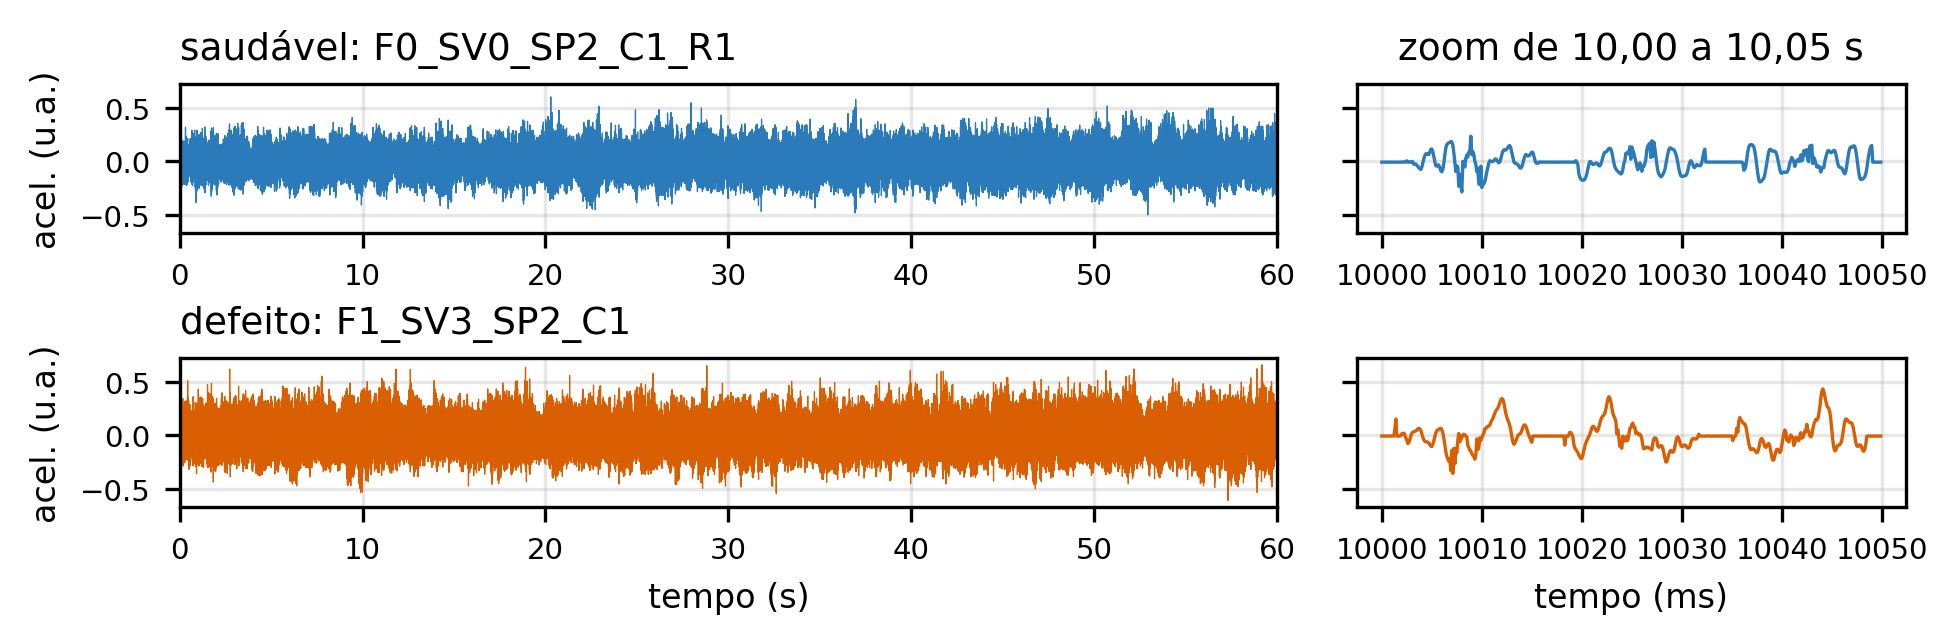
\includegraphics[width=\textwidth]{fig_tempo.png}
\caption{Aceleração no tempo em SP2 (mesma data de gravação): registro completo e trecho de 50~ms.}
\label{fig:tempo}
\end{figure}

Para cada janela $x[n]$ calculamos a média $\bar{x} = \frac{1}{N}\sum_n x[n]$, a potência média $P = \frac{1}{N}\sum_n x^2[n]$, o RMS $x_{rms} = \sqrt{P}$, o desvio padrão $\sigma = \sqrt{\frac{1}{N}\sum_n (x[n] - \bar{x})^2}$, o pico absoluto $\max_n |x[n]|$, a amplitude pico a pico $\max_n x[n] - \min_n x[n]$ e o fator de crista $\max_n |x[n]| / x_{rms}$, todas em u.a., exceto a potência (u.a.$^2$) e o fator de crista (adimensional). A potência média é a versão discreta, numa janela, de $P_x = \lim_{T \to \infty} \frac{1}{2T}\int_{-T}^{T} |x(t)|^2\,dt$~\cite[slide 42]{aula2}, e a média é o coeficiente DC $D_0$, ``a média temporal do sinal''~\cite[slide 28]{aula8}. Uma senoide tem fator de crista $\sqrt{2} \approx 1{,}41$. Os resultados estão na Tabela~\ref{tab:tempo} e na Figura~\ref{fig:boxtempo}.

\begin{table}[htbp]
\centering
\caption{Características temporais: média (desvio padrão) sobre as janelas; S é saudável e D, defeito.}
\label{tab:tempo}
\footnotesize
\setlength{\tabcolsep}{4pt}
\begin{tabular}{lcccccc}
\toprule
 & \multicolumn{2}{c}{SP1} & \multicolumn{2}{c}{SP2} & \multicolumn{2}{c}{SP3} \\
\cmidrule(lr){2-3}\cmidrule(lr){4-5}\cmidrule(lr){6-7}
Característica & S & D & S & D & S & D \\
\midrule
Média ($10^{-3}$ u.a.) & $-0{,}77$ (0,52) & $-1{,}06$ (0,26) & $-0{,}96$ (0,64) & $-1{,}18$ (0,58) & $-1{,}44$ (1,25) & $-1{,}70$ (1,64) \\
RMS (u.a.) & 0,063 (0,016) & 0,025 (0,004) & 0,129 (0,032) & 0,098 (0,015) & 0,273 (0,049) & 0,305 (0,119) \\
Potência ($10^{-3}$ u.a.$^2$) & 4,2 (2,1) & 0,65 (0,23) & 17,7 (8,6) & 9,9 (3,2) & 76,9 (26,4) & 106,8 (80,0) \\
Desvio padrão (u.a.) & 0,063 (0,016) & 0,025 (0,004) & 0,129 (0,032) & 0,098 (0,015) & 0,273 (0,049) & 0,305 (0,119) \\
Pico absoluto (u.a.) & 0,28 (0,08) & 0,13 (0,02) & 0,55 (0,15) & 0,44 (0,08) & 1,01 (0,20) & 1,11 (0,36) \\
Pico a pico (u.a.) & 0,53 (0,14) & 0,23 (0,03) & 1,01 (0,25) & 0,82 (0,12) & 1,89 (0,38) & 2,11 (0,68) \\
Fator de crista & 4,56 (0,61) & 5,43 (0,73) & 4,30 (0,57) & 4,52 (0,50) & 3,71 (0,44) & 3,76 (0,51) \\
\bottomrule
\end{tabular}
\end{table}

\begin{figure}[htbp]
\centering
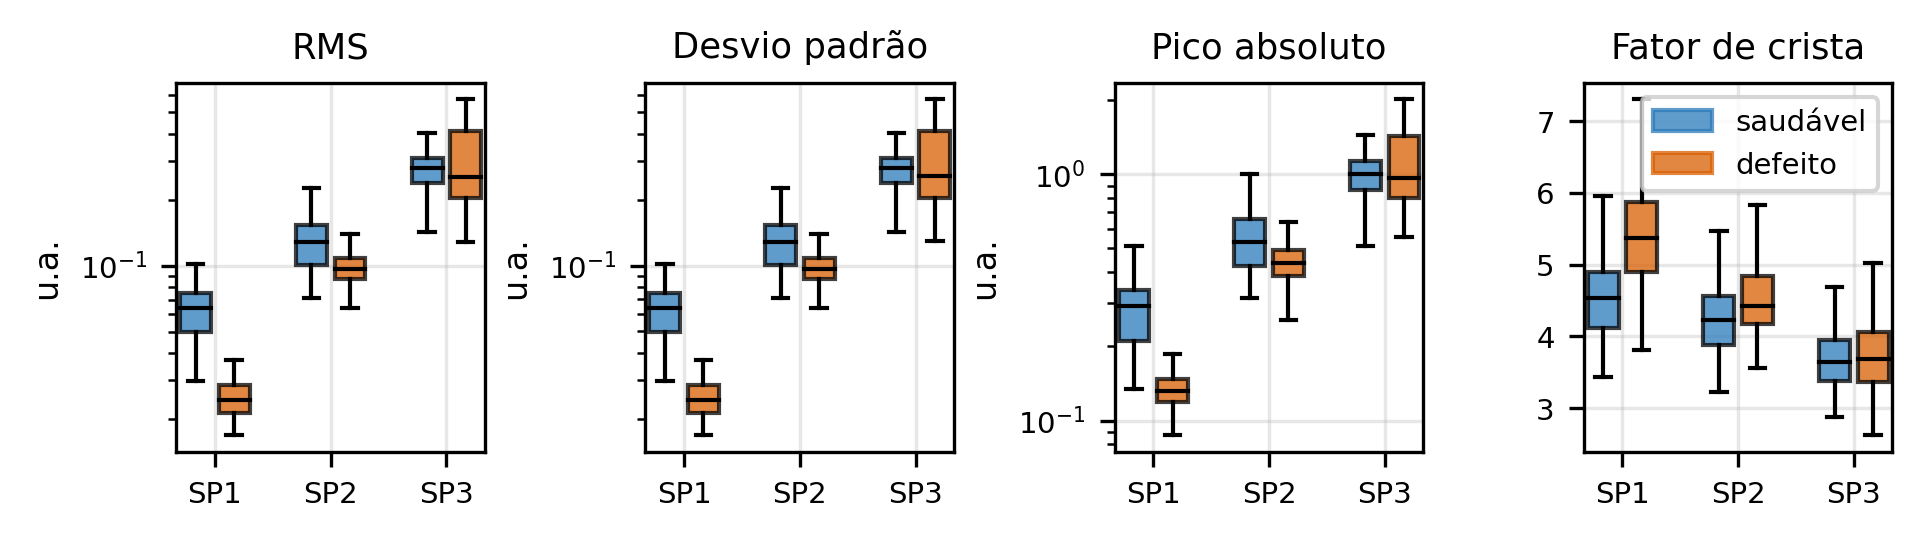
\includegraphics[width=\textwidth]{fig_box_tempo.png}
\caption{Características temporais por janela de 1~s, por velocidade e condição.}
\label{fig:boxtempo}
\end{figure}

Pela definição, $P = x_{rms}^2$, e, abrindo o quadrado em $\sigma$, $x_{rms}^2 = \bar{x}^2 + \sigma^2$. É a decomposição do teorema de Parseval para séries de Fourier, pelo qual ``a potência do sinal no domínio do tempo é igual à soma das potências das componentes no domínio da frequência''~\cite[slide 27]{aula8}: o termo $|D_0|^2$ é $\bar{x}^2$ e os demais somam a variância. As duas igualdades foram conferidas numericamente (erro de $10^{-16}$). Logo, RMS e potência carregam a mesma informação e, como a média responde por no máximo 0,66\% da potência, RMS e desvio padrão praticamente coincidem. Com um offset grande, o RMS seria inflado por um nível constante que não é vibração, e o desvio padrão seria a medida adequada. A média não distingue as condições.

A intensidade depende muito mais da velocidade do que da condição (o RMS cresce de 4 a 12 vezes entre SP1 e SP3), e o defeito não implica mais vibração: em SP1 o saudável tem RMS 2,5 vezes maior, em SP2 ainda um pouco maior, e em SP3 as classes se sobrepõem. O fator de crista, que não depende da escala, é maior no defeito, sobretudo em SP1 (5,43 contra 4,56), indicando um sinal mais impulsivo. RMS, potência, desvio padrão, pico e pico a pico medem a escala do sinal e são redundantes entre si.

\section{Análise no domínio da frequência}

\subsection{FFT, eixo de frequências e normalização}

A DFT surge de duas restrições do problema: só observamos o sinal num intervalo de duração $T_0 = N/f_s$ e só conhecemos as amostras $x[n] = x(nT)$~\cite[slide 15]{aula2}. Um sinal definido apenas num intervalo de comprimento $T_0$ pode ser escrito como série de Fourier com $\omega_0 = 2\pi/T_0$~\cite[slide 4]{aula8}, e, aproximando a integral dos coeficientes por uma soma com passo $T$,
\begin{equation}
D_k = \frac{1}{T_0}\int_0^{T_0} x(t)\,e^{-j2\pi kt/T_0}\,dt \approx \frac{1}{N}\sum_{n=0}^{N-1} x[n]\,e^{-j2\pi kn/N} = \frac{X[k]}{N},
\end{equation}
onde $X[k]$ é a DFT calculada pela FFT. Daí saem o eixo, $f_k = k/T_0 = k f_s/N$ com $\Delta f = f_s/N$, e a normalização: uma senoide $a\cos(2\pi f_k t)$ tem $D_{\pm k} = a/2$, então usamos a amplitude $A[k] = 2|X[k]|/N$ e a potência por raia $P[k] = 2|X[k]|^2/N^2$ (sem o fator 2 em $k = 0$ e em $f_s/2$), apenas em $0 \le f \le f_s/2$ por o sinal ser real. Removida a média, $\sum_k P[k] = \sigma^2$ por Parseval~\cite[slide 27]{aula8}, o que conferimos em todas as janelas; usamos janela retangular para manter essa igualdade exata.

\subsection{Espectros comparativos}

Na Figura~\ref{fig:espectros} (média das 60 janelas de cada registro em SP2), o maior pico do saudável está em 98~Hz, que interpretamos como a rotação (cerca de 5.900~rpm, coerente com as rajadas a cada 10~ms), e os demais em múltiplos inteiros dela (197, 296, 394 e 492~Hz). Os defeituosos têm a mesma estrutura deslocada para baixo: 93 a 94~Hz na rotação e 370 a 374~Hz no quarto harmônico. É o espectro de um sinal periódico: na série de Fourier $x(t) = \sum_n D_n e^{jn\omega_0 t}$, com $\omega_0 = 2\pi f_{rot}$~\cite[slide 4]{aula8}, só existem componentes em $n f_{rot}$, e cada $D_n$ é calculado sobre um único período. Assim, as posições dos picos dependem só da rotação e as alturas, da forma da vibração em uma volta. No saudável domina o primeiro harmônico; em F2 e F3 o quarto fica tão alto quanto o primeiro ou mais, e em F1 o primeiro cresce. O defeito muda, portanto, a forma da vibração em cada volta. Não atribuímos causa física aos picos que não são múltiplos da rotação.

\begin{figure}[htbp]
\centering
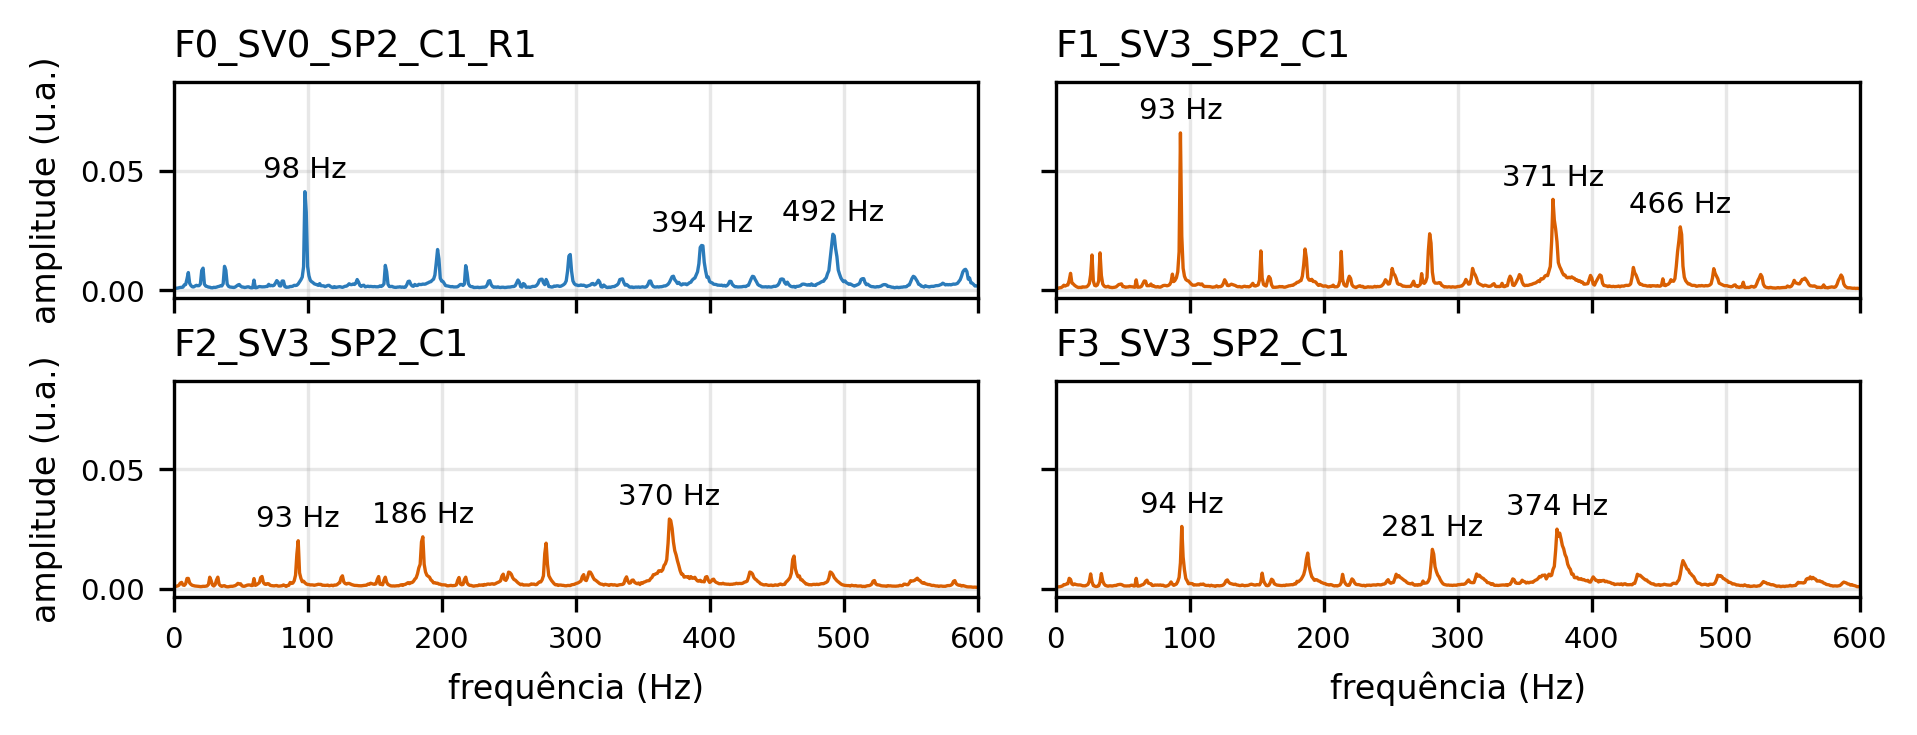
\includegraphics[width=\textwidth]{fig_espectros.png}
\caption{Espectro de amplitude médio (60 janelas de 1~s) do saudável R1 e dos três defeitos em severidade SV3, em SP2.}
\label{fig:espectros}
\end{figure}

\subsection{Características espectrais}

Por janela, extraímos a frequência dominante $f_{k^*}$, com $k^* = \arg\max_{k \ge 1} A[k]$, a magnitude $A[k^*]$ do pico, o centroide $\sum_k f_k P[k] / \sum_k P[k]$, a entropia espectral normalizada $-\sum_k p_k \log_2 p_k / \log_2 K$, com $p_k = P[k]/\sum_j P[j]$ e $K$ raias, e a potência $\sum P[k]$ em quatro bandas: B1 (0 a 200~Hz) contém a rotação nas três velocidades, B2 (200 a 500~Hz) os harmônicos de ordem 2 a 5, onde aparecem as diferenças de forma, B3 (500 a 2.000~Hz) harmônicos altos e banda larga, e B4 (2.000 a 5.000~Hz) praticamente só ruído. As bandas cobrem todo o espectro e somam $\sigma^2$ (erro relativo de $10^{-15}$), o que confirma a coerência entre as convenções do tempo e da frequência (Tabela~\ref{tab:freq} e Figura~\ref{fig:freqcar}).

\begin{table}[htbp]
\centering
\caption{Características espectrais: média (desvio padrão) sobre as janelas.}
\label{tab:freq}
\footnotesize
\setlength{\tabcolsep}{4pt}
\begin{tabular}{lcccccc}
\toprule
 & \multicolumn{2}{c}{SP1} & \multicolumn{2}{c}{SP2} & \multicolumn{2}{c}{SP3} \\
\cmidrule(lr){2-3}\cmidrule(lr){4-5}\cmidrule(lr){6-7}
Característica & S & D & S & D & S & D \\
\midrule
Freq. dominante (Hz) & 139 (95) & 135 (113) & 244 (114) & 282 (132) & 239 (129) & 249 (126) \\
Magnitude do pico (u.a.) & 0,040 (0,012) & 0,015 (0,007) & 0,079 (0,030) & 0,052 (0,016) & 0,202 (0,059) & 0,222 (0,120) \\
Centroide (Hz) & 338 (37) & 480 (94) & 410 (47) & 462 (42) & 355 (49) & 367 (60) \\
Entropia & 0,50 (0,05) & 0,61 (0,08) & 0,52 (0,05) & 0,56 (0,04) & 0,43 (0,07) & 0,44 (0,06) \\
B1 ($10^{-3}$ u.a.$^2$) & 1,4 (0,8) & 0,32 (0,21) & 4,6 (2,0) & 2,6 (1,4) & 34,8 (21,0) & 47,0 (52,0) \\
B2 ($10^{-3}$ u.a.$^2$) & 2,5 (1,6) & 0,22 (0,08) & 11,5 (7,2) & 6,0 (2,2) & 36,2 (17,0) & 53,2 (34,0) \\
B3 ($10^{-3}$ u.a.$^2$) & 0,15 (0,04) & 0,06 (0,01) & 1,1 (0,3) & 1,0 (0,3) & 4,3 (1,0) & 4,6 (3,0) \\
B4 ($10^{-3}$ u.a.$^2$) & 0,14 (0,05) & 0,04 (0,01) & 0,46 (0,20) & 0,28 (0,08) & 1,7 (0,5) & 2,0 (1,3) \\
\bottomrule
\end{tabular}
\end{table}

\begin{figure}[htbp]
\centering
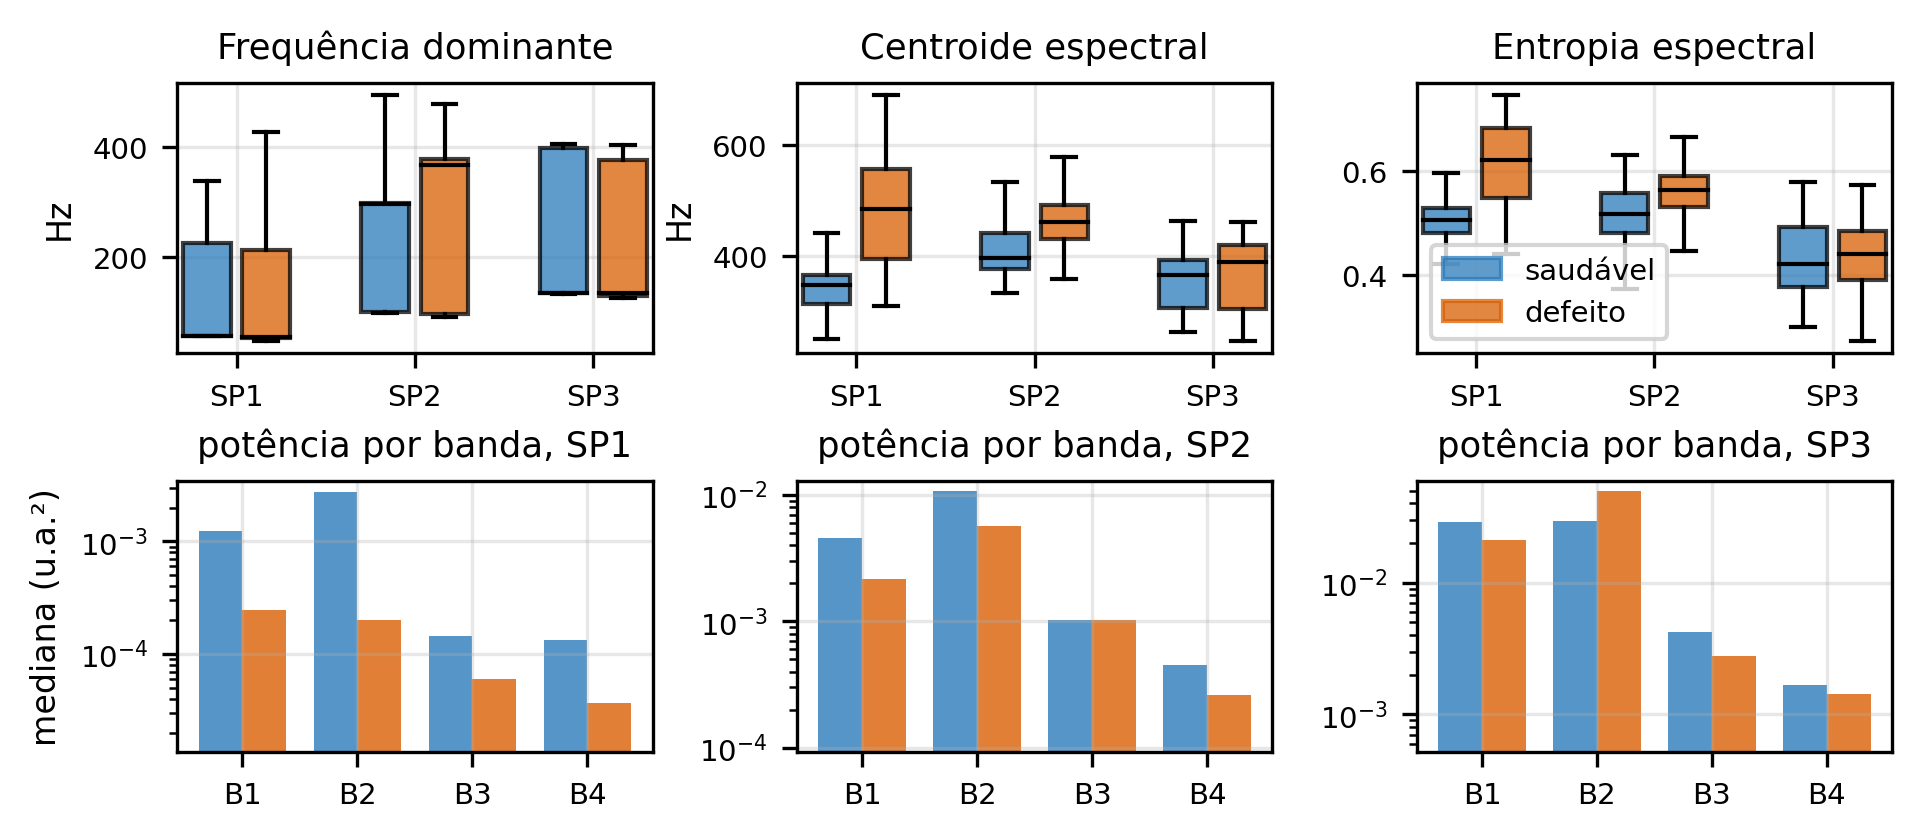
\includegraphics[width=\textwidth]{fig_freq_caract.png}
\caption{Acima, frequência dominante, centroide e entropia espectral. Abaixo, mediana da potência por banda (escala própria em cada painel).}
\label{fig:freqcar}
\end{figure}

A frequência dominante salta entre harmônicos de uma janela para outra, o que torna seu boxplot bimodal e a faz separar mal as classes. O centroide e a entropia são maiores no defeito em SP1 (480 contra 338~Hz e 0,61 contra 0,50) e em SP2, ou seja, no defeito a potência se espalha mais pelos harmônicos superiores; em SP3 as classes se sobrepõem. Nas bandas, o saudável tem mais potência em SP1 e SP2, coerente com o RMS, e em SP3 a mediana do defeito só é maior na B2.

\subsection{Resolução espectral}

Na Figura~\ref{fig:resalias}a, com 0,1~s a rotação aparece ``em 100~Hz'', a raia mais próxima de 98,5~Hz, e picos a menos de 10~Hz se fundem; com 2~s ($\Delta f = 0{,}5$~Hz) ela aparece em 98,5~Hz, e com 10~s o pico se divide em raias entre 97 e 100~Hz, porque a rotação varia levemente no trecho. O espaçamento $\Delta f = 1/T_0$ vem da série de Fourier num intervalo de duração $T_0$~\cite[slide 4]{aula8} e depende só da duração, não da taxa de amostragem. O alargamento dos picos vem do recorte: o produto por um retângulo, de transformada $T_0\,\mathrm{sinc}(\omega T_0/2)$~\cite[slide 8]{aula10}, vira $\frac{1}{2\pi}(F_1 * F_2)(j\omega)$ na frequência~\cite[slide 3]{aula11}, então cada raia vira uma sinc de largura inversamente proporcional a $T_0$, pois ``o pulso estreito produz uma transformada larga e um pulso largo produz um espectro estreito''~\cite[slide 10]{aula10}. A janela de 1~s resolve os 4~Hz entre saudável e defeito sem que a rotação varie dentro dela.

\begin{figure}[htbp]
\centering
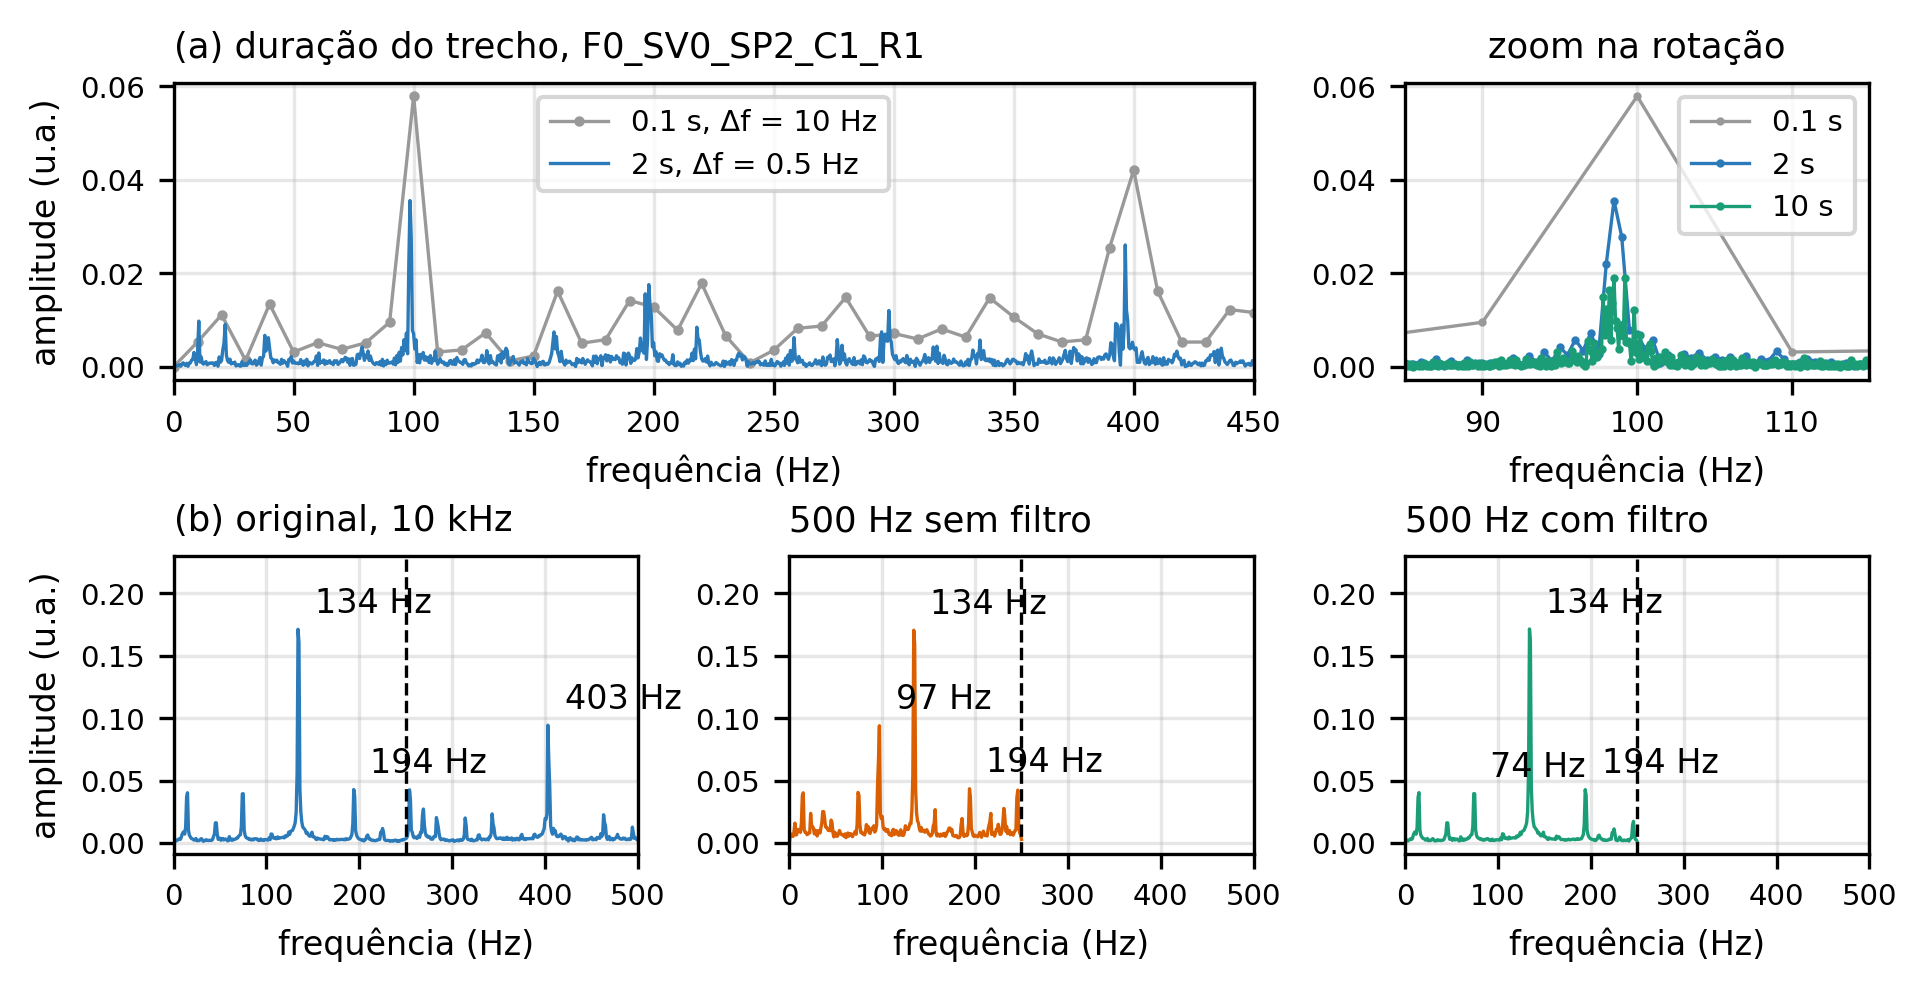
\includegraphics[width=\textwidth]{fig_res_alias.png}
\caption{(a) Efeito da duração do trecho no espectro do saudável em SP2, com zoom na rotação. (b) Espectro do saudável em SP3 a 10~kHz e reamostrado a 500~Hz sem e com filtro anti-aliasing; a linha tracejada marca 250~Hz.}
\label{fig:resalias}
\end{figure}

\subsection{Amostragem e aliasing}

Reduzimos a taxa de 10~s do saudável em SP3, com picos em 134 e 403~Hz, para $f_s' = 500$~Hz (Nyquist de 250~Hz), guardando uma amostra a cada 20: $x_d[n] = x[20n]$, o escalamento no tempo discreto ou decimação~\cite[slide 18]{aula2} (Figura~\ref{fig:resalias}b). Como a amostragem ideal é o produto por um trem de impulsos~\cite[slide 30]{aula3}, pela convolução na frequência~\cite[slide 3]{aula11} o espectro amostrado é o original repetido a cada $f_s'$, e componentes acima de $f_s'/2$ fazem as cópias se sobreporem. Assim, o pico de 403~Hz reaparece em $500 - 403 = 97$~Hz sem filtro, onde o original não tem nada, e poderia ser confundido com a rotação de SP2. Com um passa-baixas aplicado antes, que idealmente ``suprime todas as frequências acima de uma frequência de corte''~\cite[slide 16]{aula12} e atua como $Y(j\omega) = H(j\omega)X(j\omega)$~\cite[slide 4]{aula12}, o pico falso some e a faixa de 0 a 250~Hz fica igual à original. Analisar até o quinto harmônico em SP3 (cerca de 670~Hz) exige $f_s > 1{,}3$~kHz, o que exclui a IMU.

\section{Comparação entre os domínios}

Para comparar características de unidades diferentes, usamos a diferença entre as médias das classes em desvios padrão, $d = (\mu_{D} - \mu_{S}) / \sqrt{(\sigma_{D}^2 + \sigma_{S}^2)/2}$, por velocidade e sobre as janelas de cada classe (Figura~\ref{fig:separacao}). Com $d$ perto de zero as classes se sobrepõem, e com $|d|$ por volta de 2 quase não se sobrepõem.

\begin{figure}[htbp]
\centering
\begin{minipage}[c]{0.52\textwidth}
\centering
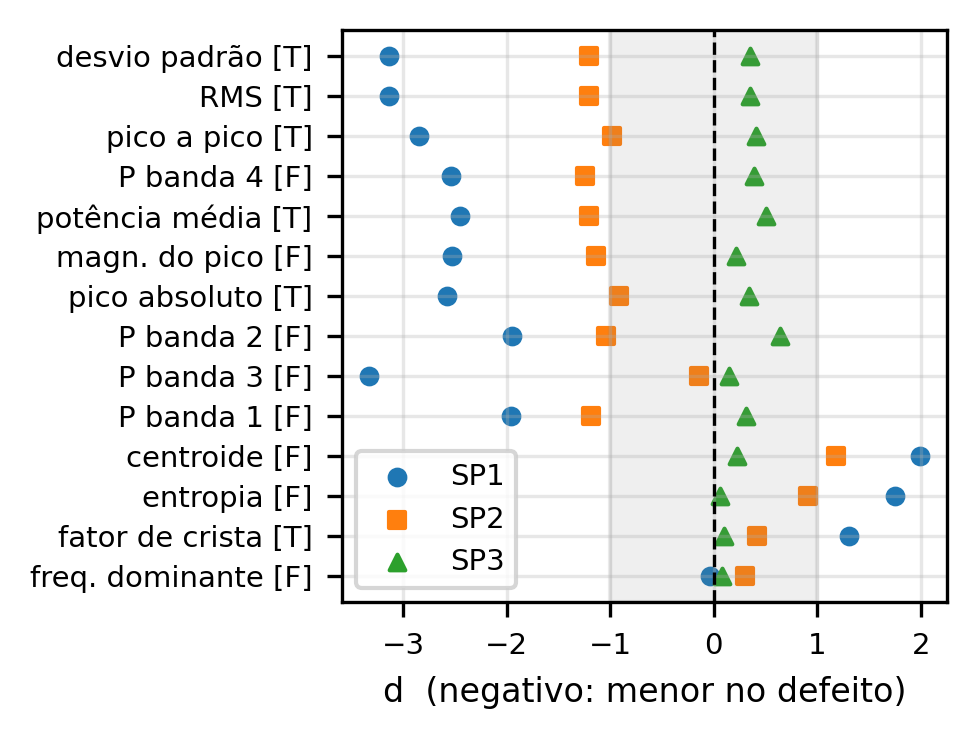
\includegraphics[width=\textwidth]{fig_separacao.png}
\end{minipage}\hfill
\begin{minipage}[c]{0.44\textwidth}
\caption{Separação $d$ entre defeito e saudável por característica e velocidade ([T] tempo, [F] frequência). Valores negativos indicam característica menor no defeito, e a faixa cinza marca $|d| < 1$.}
\label{fig:separacao}
\end{minipage}
\end{figure}

O primeiro achado é que a intensidade separa as classes, mas depende da velocidade e vai na direção contrária à esperada: RMS, desvio padrão, pico e pico a pico têm $d$ entre $-2{,}6$ e $-3{,}1$ em SP1 (menores no defeito), cerca de $-1$ em SP2 e entre 0,3 e 0,4 em SP3, e $d \approx -0{,}1$ com as velocidades juntas. O segundo é que a frequência mostra o que o tempo não mostra: o centroide ($d$ = 2,0 e 1,2 em SP1 e SP2) e a entropia (1,75 e 0,91) separam melhor que o fator de crista (1,3 e 0,42), a melhor medida temporal independente da escala; o centroide mantém $d = 0{,}97$ com as velocidades misturadas; e só o espectro revela a rotação mais baixa do defeito. Em SP3 nenhuma característica isolada separa bem ($|d| \le 0{,}64$), então nenhum domínio é superior em todas as condições.

Pela correlação de Spearman, RMS, potência e desvio padrão são equivalentes ($\rho = 1{,}00$), e pico, pico a pico, magnitude do pico e bandas acompanham o RMS ($\rho \ge 0{,}95$), enquanto fator de crista, centroide, entropia e frequência dominante trazem informação diferente ($|\rho| \le 0{,}80$). Para a classificação propomos RMS, pico absoluto e fator de crista no tempo e B1, B2, centroide, entropia e frequência dominante na frequência, tratando a velocidade de forma explícita.

\section{Investigação adicional}

Perguntamos como a velocidade modifica os picos espectrais e se a diferença entre as condições se mantém nas três velocidades. Se a hélice gira $a$ vezes mais rápido com a mesma forma de vibração por volta, o sinal vira $x(at)$~\cite[slide 17]{aula2}, e pelo teorema do escalamento $f(at) \leftrightarrow \frac{1}{|a|}F(j\omega/a)$~\cite[slide 7]{aula10}: o espectro se estica pelo mesmo fator. Estimamos então a rotação $f_{rot}$ de cada registro, como o maior pico numa faixa em torno da rotação de cada velocidade, e redesenhamos os espectros em função da ordem $f/f_{rot}$ (Figura~\ref{fig:investigacao}).

\begin{figure}[htbp]
\centering
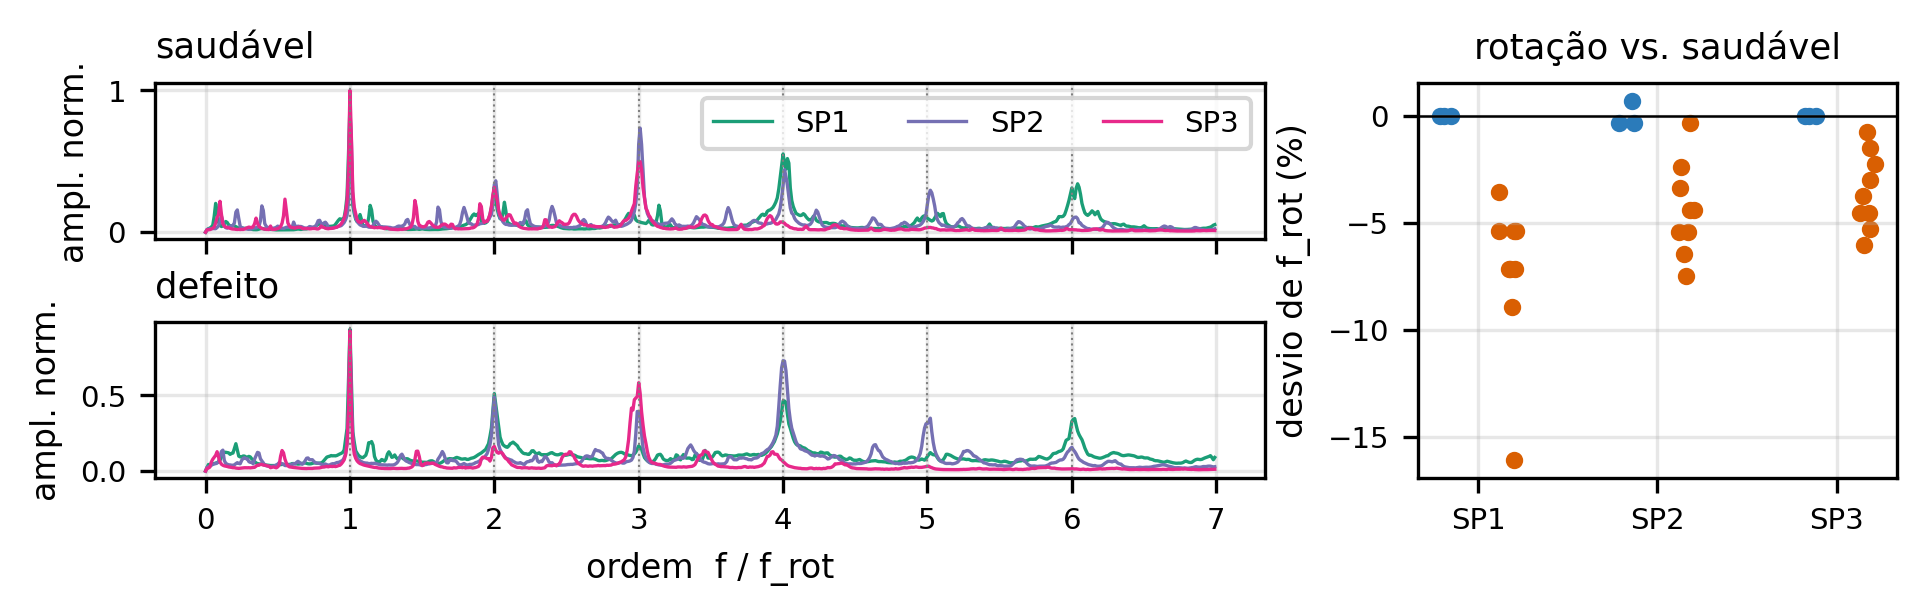
\includegraphics[width=0.94\textwidth]{fig_investigacao.png}
\caption{À esquerda, espectros médios normalizados pela ordem $f/f_{rot}$. À direita, desvio da rotação de cada registro em relação à média saudável (azul, saudável; laranja, defeito).}
\label{fig:investigacao}
\end{figure}

Nas duas classes e nas três velocidades os picos caem nas ordens inteiras, o que confirma o escalamento das posições, embora as alturas relativas mudem com a velocidade. O resultado mais claro é a rotação: em C1, 26 dos 27 defeituosos giram mais devagar que todos os saudáveis, com desvios medianos de $-7{,}1\%$, $-4{,}4\%$ e $-3{,}8\%$, e em C2 o efeito se repete em 23 de 27 registros, exceto no F1 mais leve. Como as três repetições saudáveis têm a mesma rotação apesar das datas diferentes, o efeito não parece vir da sessão de ensaio. Assim, só a rotação mais baixa do defeito se mantém nas três velocidades e nas duas configurações, e os dados não permitem dizer por quê.

\section{Conclusão}

No tempo, as medidas de intensidade são redundantes, dependem sobretudo da velocidade e não indicam mais vibração no defeito, e só o fator de crista descreve a forma do sinal. Na frequência, o defeito redistribui a potência entre os harmônicos e gira um pouco mais devagar em todas as velocidades.

\begin{thebibliography}{9}
\bibitem{dataset} M. A. A. Ismail, M. E. Elshaar, A. Abdalla e Q. Quan. \textit{DronePropB: Ground Testing Dataset for Commercial Drones with Defective Propellers}. Mendeley Data, V1, 2024. DOI: \href{https://doi.org/10.17632/xkvfjmm8zg.1}{10.17632/xkvfjmm8zg.1}.
\bibitem{aula1} D. R. Campelo. \textit{Lecture 1: Introduction to the course}. Notas de aula de CIN0020 Sinais e Sistemas, CIn-UFPE, 2026.
\bibitem{aula2} D. R. Campelo. \textit{Lecture 2: Signal Characteristics and Models}. Notas de aula de CIN0020 Sinais e Sistemas, CIn-UFPE, 2026.
\bibitem{aula3} D. R. Campelo. \textit{Lecture 3: Signal Models}. Notas de aula de CIN0020 Sinais e Sistemas, CIn-UFPE, 2026.
\bibitem{aula8} D. R. Campelo. \textit{Lecture 8: Continuous-Time Fourier Series}. Notas de aula de CIN0020 Sinais e Sistemas, CIn-UFPE, 2026.
\bibitem{aula10} D. R. Campelo. \textit{Lecture 10: Fourier Transform Properties}. Notas de aula de CIN0020 Sinais e Sistemas, CIn-UFPE, 2026.
\bibitem{aula11} D. R. Campelo. \textit{Lecture 11: Fourier Theorems and Generalized Fourier Transforms}. Notas de aula de CIN0020 Sinais e Sistemas, CIn-UFPE, 2026.
\bibitem{aula12} D. R. Campelo. \textit{Lecture 12: Frequency Response of LTI Systems}. Notas de aula de CIN0020 Sinais e Sistemas, CIn-UFPE, 2026.
\end{thebibliography}

\end{document}
